\documentclass{beamer}
\usepackage[utf8]{inputenc}
\usepackage[T1]{fontenc}

\hypersetup{
	colorlinks,
	allcolors=.,
	urlcolor=blue,
}

\title{Linux, Unix\\ et OpenSource}
\date{16/12/2022}
\author[JB Boni]{\href{https://github.com/Odonon}{Jean-Baptiste Boni}\\D'après un travail collaboratif avec\\ \href{https://github.com/NicolasFlandrois}{Nicolas Flandrois}}

\usetheme[]{ecamrs}

\begin{document}

\begin{frame}[plain]
\titlepage
\end{frame}

%\begin{frame}[plain]{Table of contents}
%	\tableofcontents
%\end{frame}



\section[Logiciel libre]{Logiciel libre : définitions et grandes figures}

\subsection{Les grandes figures du logiciel libre}
\begin{frame} 
\frametitle{Story Time !} 

\begin{center}
	Comment en suis-je arrivé là ?

	\begin{tikzpicture}
		\node[] (avant) {\includegraphics[width=6cm,trim={4cm 7cm 9cm 0},clip]{static/img/JB_2017.jpg}};
	\end{tikzpicture}
\end{center}

\end{frame}

\begin{frame}
	\frametitle{Richard Stallman}
	
\begin{columns}
	\begin{column}{.5\textwidth}
		Think free speech not free beer
	\end{column}
	
	
	\begin{column}{.5\textwidth}
		\href{https://fr.wikipedia.org/wiki/Richard_Stallman}{\includegraphics[width=5cm]{static/img/richard_stallman.jpeg}}
	\end{column}
\end{columns}
\end{frame}

\begin{frame}
	\frametitle{Linus Torvalds}
	
\begin{columns}
	\begin{column}{.3\linewidth}
		\href{https://fr.wikipedia.org/wiki/Linus_Torvalds}{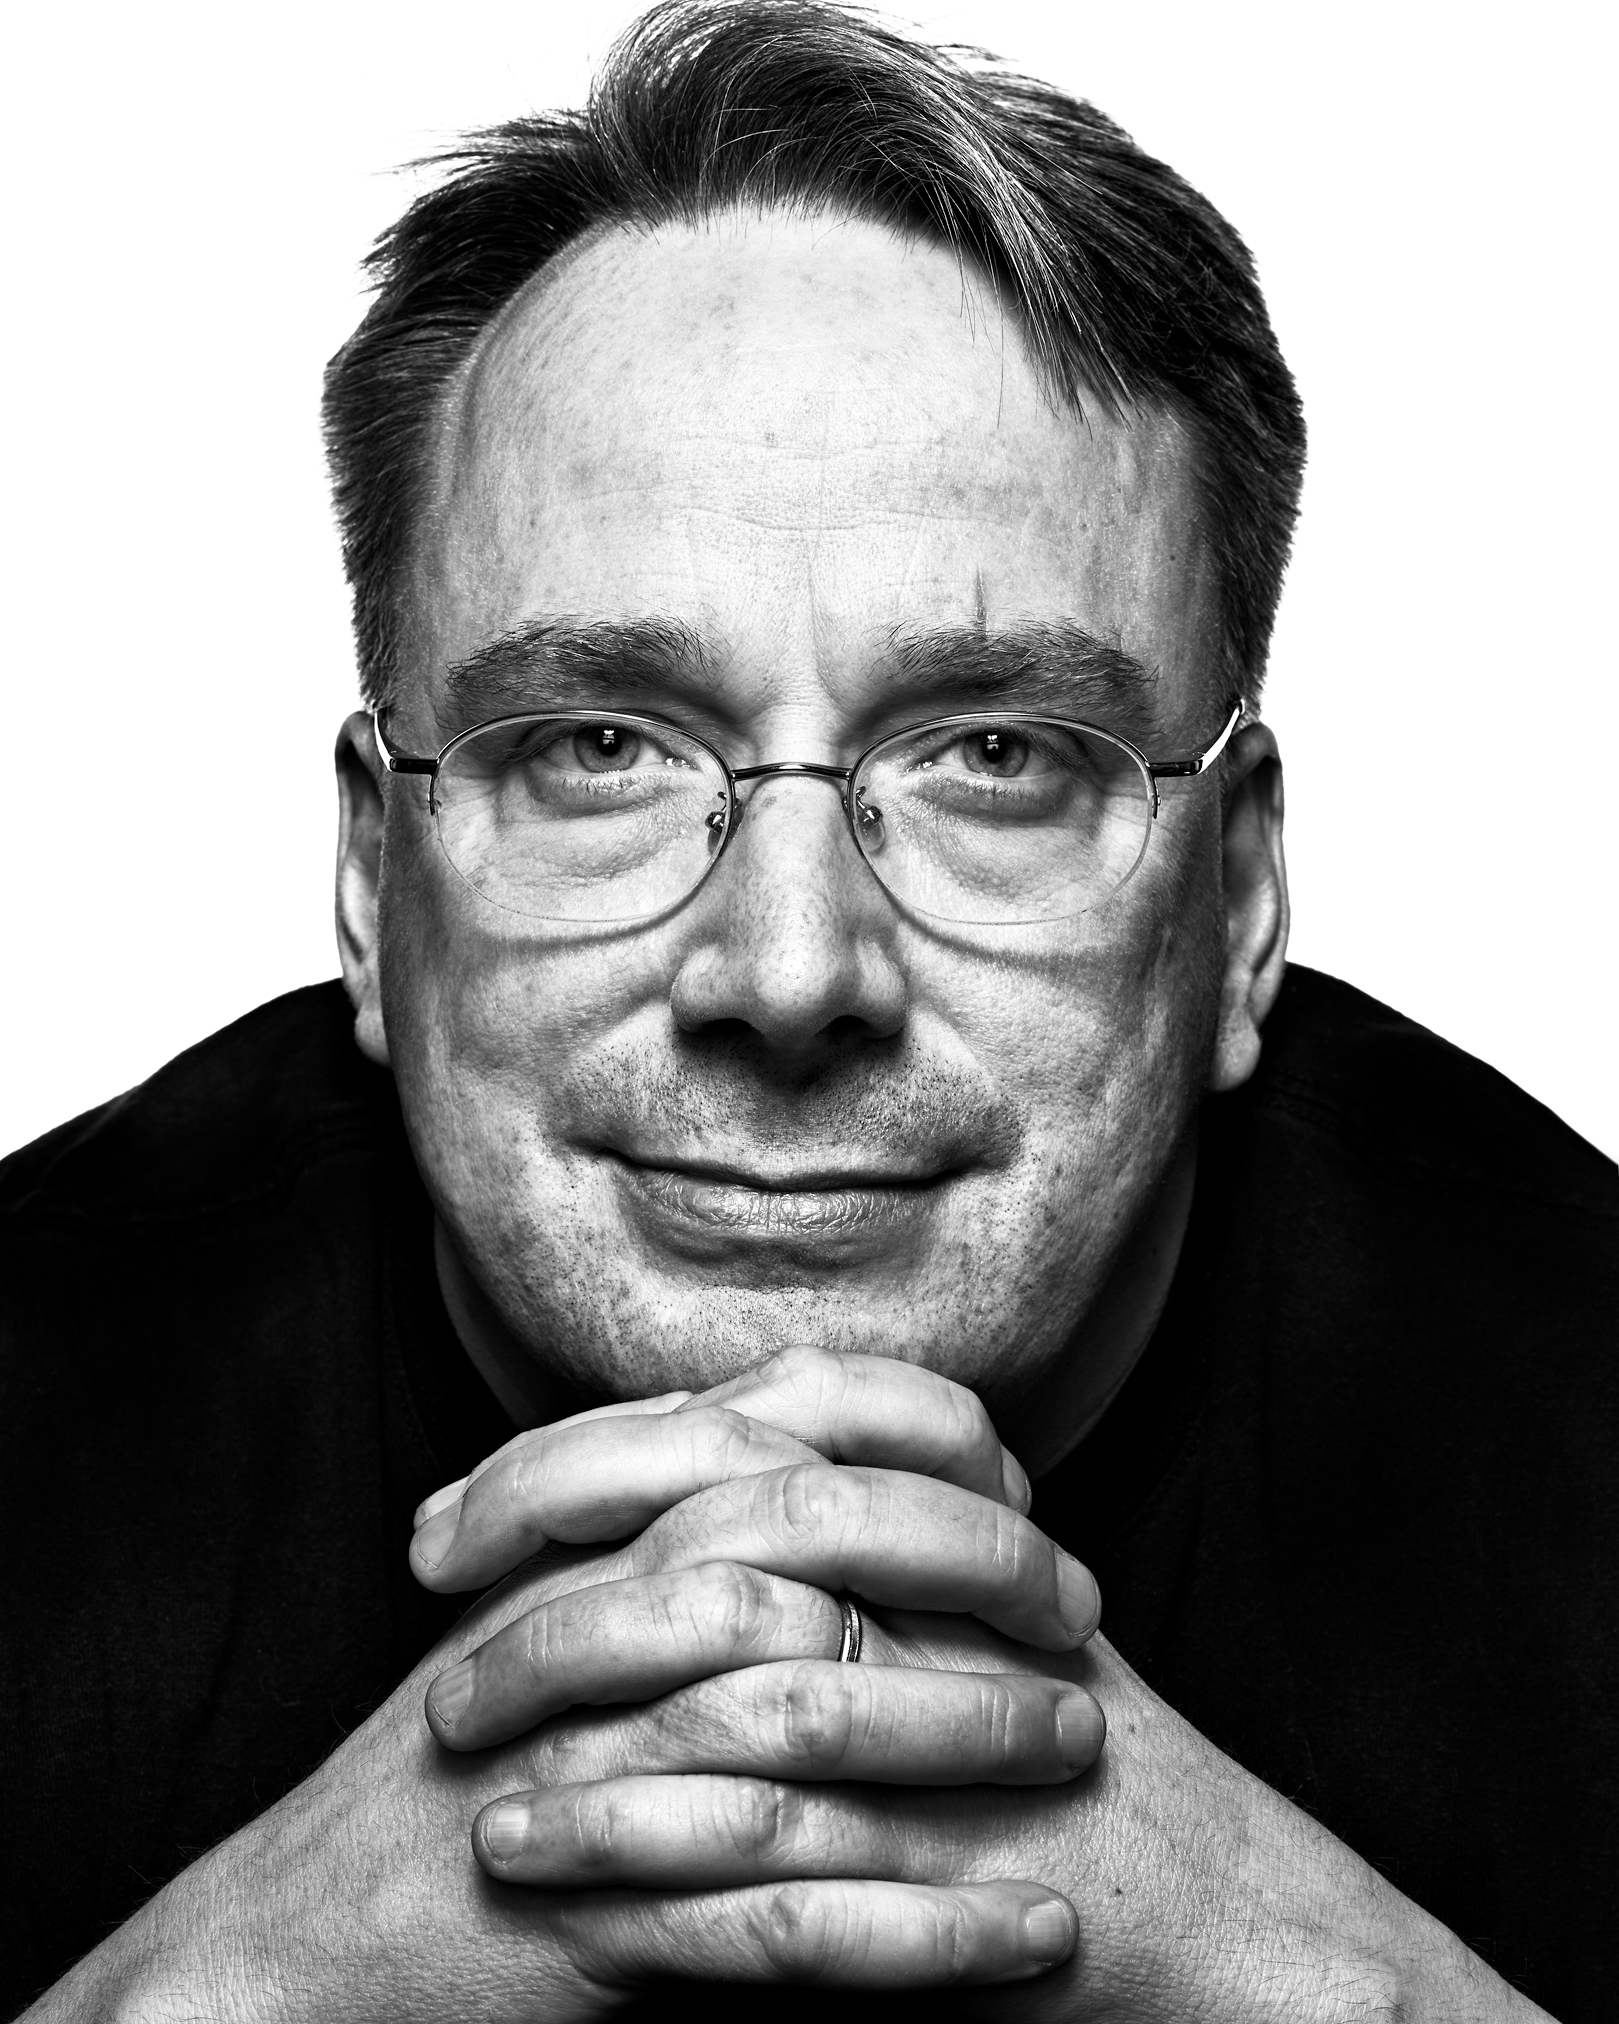
\includegraphics[width=3cm]{static/img/linus_torvalds.jpg}}
	\end{column}

	\begin{column}{.7\linewidth}
		\begin{itemize}
			\item 1990 -- Début de ses travaux sur le \href{https://github.com/torvalds/linux}{Kernel Linux}.
			\item 1991 -- Publication du premier prototype du Kernel.
			\item 2005 -- Création du logiciel de versionning maison \href{https://git-scm.com/}{Git}, utilisé par le gestionnaire de dépôt \href{https://github.com/}{Github}.
			\item Honoré par de nombreux prix à travers le monde.
		\end{itemize}
	\end{column}
\end{columns}
	
\end{frame}

\subsection{Logiciel libre, entre philosophie et culture internet}
\begin{frame}
	\frametitle{\insertsubsection}
	\begin{tikzpicture}
		\node[draw,align=center] (GNU) {
\includegraphics[width=4cm]{static/img/GNU_white.png}\\ \href{https://fr.wikipedia.org/wiki/Logiciel_libre}{GNU Project}};
		\node[draw,align=center] (open) at ++(7,0) {\includegraphics[width=4cm]{static/img/open-source.png}\\ \href{https://fr.wikipedia.org/wiki/Open_source}{Open Source Initiative}};
		\draw[->,very thick] (GNU)--(open) node[midway,above]{?};
	\end{tikzpicture}
\end{frame}

\begin{frame}
	\frametitle{Internet: un cas concret dans l'histoire}
	
	A qui appartient Internet et son contenu ?
	
	\begin{itemize}
		\item<2-> Aux états ?
		\item<3-> A des entreprises ?
		\item<4-> A tout le monde ?
	\end{itemize}

	\vspace{2em}
	\uncover<5->{Ecosystème des hackers (\href{https://fr.wikipedia.org/wiki/Manifeste_du_hacker}{Hackers Manifesto})}
	
	\begin{flushright}
	\uncover<6->{\href{https://en.wikipedia.org/wiki/A_Declaration_of_the_Independence_of_Cyberspace}{Déclaration d'indépendance du cyberespace -- P.Barlow}}
	\end{flushright}
\end{frame}

\begin{frame}
	\frametitle{Déclaration d'indépendance du cyberespace}
	
	Governments of the Industrial World, you weary giants of flesh and steel, I come from Cyberspace, the new home of Mind. On behalf of the future, I ask you of the past to leave us alone. You are not welcome among us. You have no sovereignty where we gather.
	
	\vspace{2em}
	
	Gouvernements du monde industriel, géants fatigués de chair et d’acier, je viens du cyberespace, nouvelle demeure de l’esprit. Au nom de l’avenir, je vous demande, à vous qui êtes du passé, de nous laisser tranquilles. Vous n’êtes pas les bienvenus parmi nous. Vous n’avez aucun droit de souveraineté sur nos lieux de rencontre.
	
\end{frame}

\section{Les licences libres}

\subsection{Licences libres: contenus et utilisation}
\begin{frame}
	\frametitle{\insertsubsection}
	
	\begin{block}{Licence libre}
		Licence donnant le droit à l'utilisateur de modifier et redistribuer le logiciel. Ces licences s'appliquent au code source ainsi qu'aux formes binaires de ces logiciels.
	\end{block}

	\begin{itemize}
		\item<2-> \href{https://www.gnu.org/licenses/gpl-3.0.fr.html}{GNU General Public License (GPL) - version 3}
		\item<3-> \href{https://apache.org/licenses/}{Apache License - version 2.0}
		\item<4-> \href{https://mit-license.org/}{MIT License}
		\item<5-> et toutes les autres! (Licence BSD, CeCILL, Mozilla Public License, Open Hardware, IBM Public License, Python Software Foundation License...)
	\end{itemize}
	
\end{frame}

\begin{frame}
	\frametitle{Un peu de philo}
	{\LARGE\centering Mais, du coup, à qui ça appartient?}
\end{frame}

\begin{frame}
	\frametitle{Des enjeux politiques}
	
	\includegraphics[width=.45\linewidth]{static/img/open-source.png} \hfill 
\includegraphics[width=.45\linewidth]{static/img/nsa.png}
	
\end{frame}


\subsection{Quelques modèles économiques}
\begin{frame}
	\frametitle{\insertsubsection}
	
	\begin{columns}
		\begin{column}{.5\linewidth}
			\href{https://www.redhat.com/fr}{\includegraphics[width=\linewidth]{static/img/Red_hat_logo.png}}
			\href{https://www.adafruit.com/}{\includegraphics[width=\linewidth]{static/img/adafruit_grey.png}}
			\href{https://circuitpython.org/}{\includegraphics[width=\linewidth]{static/img/CircuitPython.png}}
		\end{column}
	
		\begin{column}{.5\linewidth}
			\href{https://system76.com/}{\includegraphics[width=.7\linewidth]{static/img/System76.jpg}}
			\href{https://pop.system76.com/}{\includegraphics[width=.7\linewidth]{static/img/POPosLinux.png}}
		\end{column}
	\end{columns}
\end{frame}

\begin{frame}
	\frametitle{Alternatives libres}
	
	Quelques exemples de logiciels libres et leurs pendant propriétaires:
	
	\begin{center}
		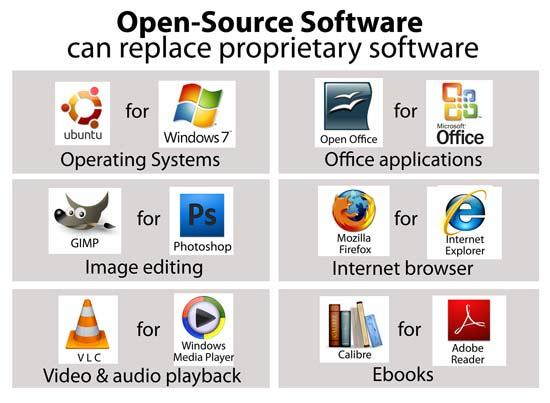
\includegraphics[width=.7\linewidth]{static/img/alternatives_libres.jpg}
	\end{center}
\end{frame}

\begin{frame}
	\frametitle{Alternatives libres}
	
	Quelques exemples pour remplacer la suite Adobe:
	
	\begin{center}
		\includegraphics[width=.8\linewidth]{static/img/open-vs-closed-Adobe.jpg}
	\end{center}
	
\end{frame}

\begin{frame}
	\frametitle{Un cas particulier exceptionnel}
	
	\begin{center}
		\href{https://www.blender.org/}{
\includegraphics[width=.55\linewidth]{static/img/Blender.png}}
	\end{center}
	
\end{frame}

\section{Et Linux dans tout ça?}

\subsection{Présentation de Linux}
\begin{frame}
	\frametitle{\insertsection}
	\begin{center}
		\href{https://fr.wikipedia.org/wiki/Linux}{\includegraphics[width=\linewidth]{static/img/logo-linux.png}}
	\end{center}
\end{frame}

\begin{frame}
	\frametitle{Un peu de vocabulaire}
	
	\begin{block}<2->{Kernel}
		Le noyau de l'operating system (OS). Il contient les principales instructions permettant de faire fonctionner l'ordinateur.
	\end{block}

	\begin{block}<3->{Distribution}
		Aussi appelée "distro", elle permet d'utiliser les instructions disponibles dans le Kernel et les modifier si nécessaire pour un besoin particulier.
	\end{block}

	\begin{block}<4->{Desktop Environnement}
		C'est la mise en page de votre distribution. C'est comme les goûts et les couleurs...
	\end{block}
	
\end{frame}

\begin{frame}
	\frametitle{Historique simplifié de Unix et ses dérivés...}
	
	\begin{center}
		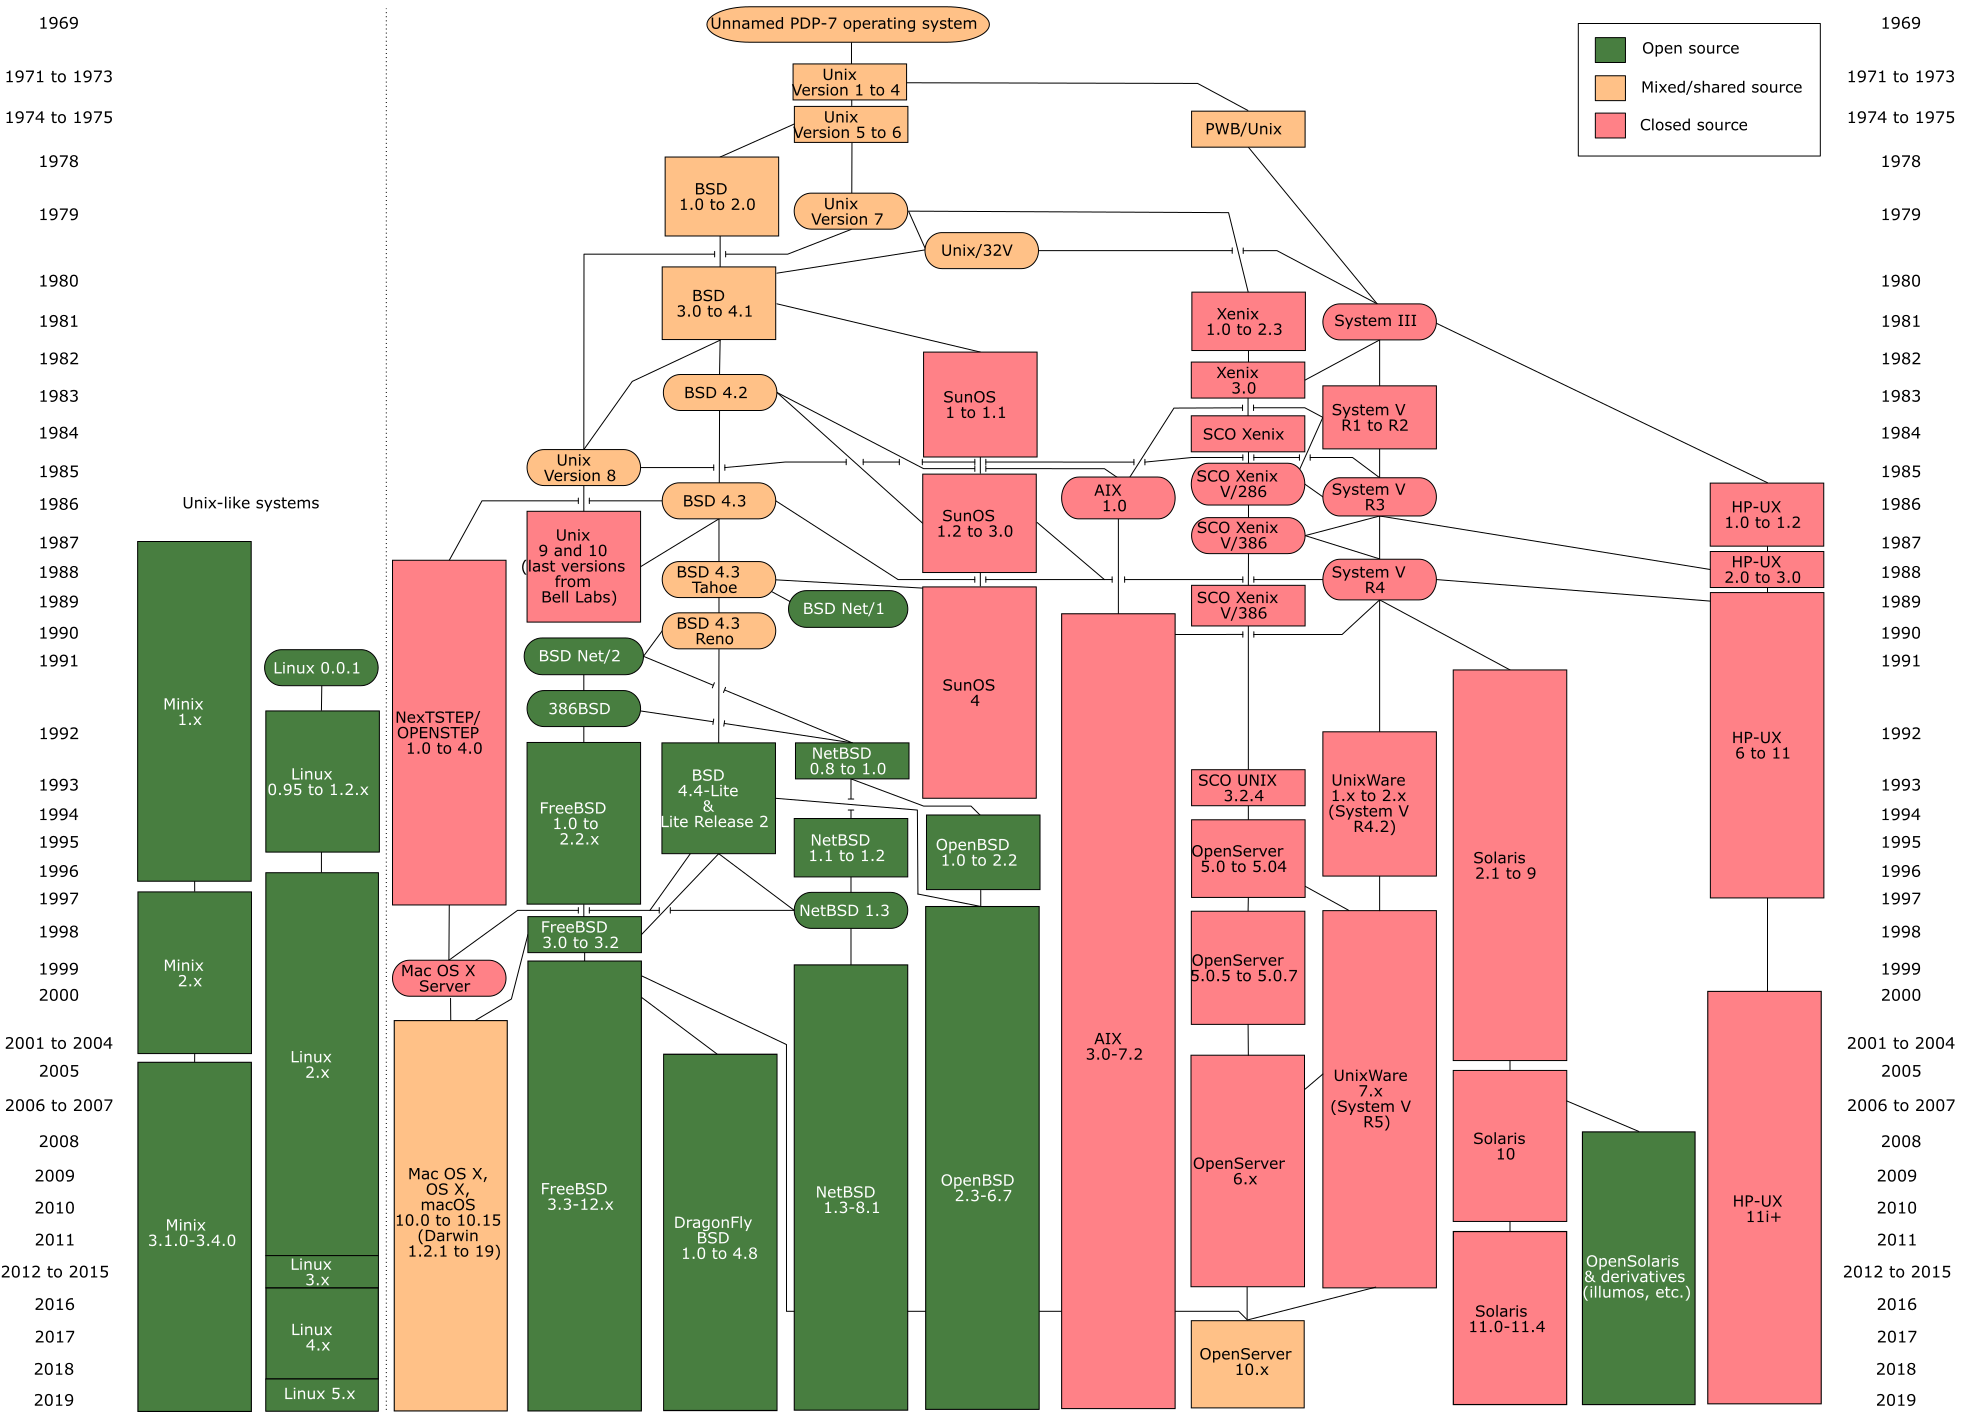
\includegraphics[width=\linewidth]{static/img/Unix_history-simple.png}
	\end{center}
\end{frame}

\begin{frame}
	\begin{center}
		Linux Kernel vs GNU Linux
		
		\includegraphics[width=.6\linewidth]{static/img/gnulinuxLogo2.png}
	\end{center}
\end{frame}

\subsection{Les distro Linux}

\begin{frame}
	\frametitle{Les grandes sœurs}
	
	\begin{center}
		\includegraphics[width=.8\linewidth]{static/img/linux_distros.png}
	\end{center}
\end{frame}

\begin{frame}
	\frametitle{La famille nombreuse}
	
	\begin{center}
		\href{https://upload.wikimedia.org/wikipedia/commons/b/b5/Linux_Distribution_Timeline_21_10_2021.svg}{\includegraphics[width=3cm,angle=-90]{static/img/linux_timeline.png}}
	\end{center}
\end{frame}

\begin{frame}
	\frametitle{One of us...}
	
	{\LARGE Linux est partout. Linux est invisible.}
	
	{\Large Vous utilisez Linux sans vous en rendre compte.}
	
\end{frame}

\begin{frame}
	\frametitle{Android}
	\begin{columns}
		\begin{column}{.5\linewidth}
			\href{https://www.android.com/intl/fr_fr/}{\includegraphics[width=\linewidth]{static/img/Android_robot_logo.png}}
		\end{column}
	
		\begin{column}{.5\linewidth}
			\href{https://www.tutorialspoint.com/android/android_architecture.htm}{\includegraphics[width=\linewidth]{static/img/android_stack.png}}
		\end{column}
	\end{columns}
\end{frame}

\begin{frame}
	\frametitle{Mais aussi...}
	\begin{itemize}
		\item<1-> Tyzen, Wearable OS
		\item<2-> Les distro mobiles
	
	\uncover<3->{\href{https://lineageos.org/}{\includegraphics[width=.45\linewidth]{static/img/Lineage_OS_Logo.png}}}
	\uncover<4->{\href{https://lineageos.org/}{\includegraphics[width=.45\linewidth]{static/img/pine_phone.png}}}
	
		\item<5-> Android Automotive et bien d'autres...
	
	\end{itemize}
	
\end{frame}

\begin{frame}
	\frametitle{Et si je veux commencer ?}
	
	\begin{columns}
		\begin{column}{.5\linewidth}
			\centering
			\href{https://linuxmint.com/}{\includegraphics[width=.5\linewidth]{static/img/Linux_Mint.png}}
			
			\href{https://ubuntu.com/download}{\includegraphics[width=.5\linewidth]{static/img/Ubuntu-old.png}}
		\end{column}
	
		\begin{column}{.5\linewidth}
			\centering
			\href{https://pop.system76.com/}{\includegraphics[width=.8\linewidth]{static/img/POPOSLinux.png}}
			
			\href{https://manjaro.org/}{\includegraphics[width=.8\linewidth]{static/img/manjaro-logo.png}}
		\end{column}
	\end{columns}
\end{frame}

\begin{frame}
	\frametitle{Mentions honorables}
	
		\begin{columns}
		\begin{column}{.5\linewidth}
			\centering
			\href{https://retropie.org.uk/}{\includegraphics[width=.7\linewidth]{static/img/retropie-logo.png}}
			
			\href{https://www.raspberrypi.com/software/}{\includegraphics[width=.5\linewidth]{static/img/RaspberryPi_Logo.png}}
		\end{column}
		
		\begin{column}{.5\linewidth}
			\centering
			\href{https://www.ros.org/}{\includegraphics[width=.6\linewidth]{static/img/Robot_OS_ROS.png}}
			
			\href{https://chimeraos.org/}{
\includegraphics[width=.5\linewidth]{static/img/chimeraos.png}}
		\end{column}
	\end{columns}
\end{frame}

\section{Pour aller plus loin}

\begin{frame}
	\centering
	\href{https://www.oshwa.org/}{\includegraphics[width=.6\linewidth]{static/img/Open-source-hardware-logo.png}}
\end{frame}

\begin{frame}
	\includegraphics[width=.3\linewidth]{static/img/adafruit_grey.png}\hfill
	\href{https://www.arduino.cc/}{\includegraphics[width=.3\linewidth]{static/img/Arduino_Logo.png}}\hfill
	\includegraphics[width=.3\linewidth]{static/img/RaspberryPi_Logo.png}
\end{frame}

\begin{frame}
	\frametitle{Tout n'est pas gagné}
	\centering
	{\LARGE \href{https://en.wikipedia.org/wiki/Electronics_right_to_repair}{Right to repair mouvement}}
	
\end{frame}

\section*{}

\begin{frame}
	\titlepage
\end{frame}

\end{document}